%---------------------------------------------------------------------
% TJAA - Example Article - Example.tex
%
% This file format has been adapted from Springer's llncs proc package.
%
% Producer: Springer
% Adapted by Sinan Kaan Yerli, ODTU Fizik Bolumu, Ekim 2010.
%
% Version: 2015-06-15 - 1.1
% Version: 2019-08-01 - 2.0
% Version: 2021-04-01 - 2.1
% Version: 2022-01-01 - 2.2
% 	- added Example-Turkce file using \TRlang
% 	  which explains multi language abstract
% 	- updated explanations in manuscript meta-data notes
% 	- added sections: Astro. Macros, Astro. Journals
% 	- added description for new columntypes
% 	- added section for auth-year commands
% Version: 2022-01-22 - 2.3
%	- added Disclosure section
% Version: 2024-09-01 - 2.4
%	- updated author & address usage with new commands
%	- updated abstract description
%	- updated keyword description
%	- added descr. for new astronomical macros
%---------------------------------------------------------------------
\documentclass[usenatbib]{tjaa}

% 用於Table
\usepackage{array}
\usepackage{tabularx}
\usepackage{booktabs}

\usepackage{amsmath} % 用于数学公式
\usepackage{listings} % 代碼塊宏包
\usepackage{color} % 代碼高亮

\definecolor{dkgreen}{rgb}{0,0.6,0}
\definecolor{gray}{rgb}{0.5,0.5,0.5}
\definecolor{mauve}{rgb}{0.58,0,0.82}

% 设置代码样式
\lstset{ %
    %language=Octave,                % the language of the code
    basicstyle=\footnotesize\ttfamily,           % the size of the fonts that are used for the code
    numbers=none,                   % where to put the line-numbers
    numberstyle=\tiny\color{gray},  % the style that is used for the line-numbers
    stepnumber=2,                   % the step between two line-numbers. If it's 1, each line 
                                    % will be numbered
    numbersep=3pt,                  % how far the line-numbers are from the code
    backgroundcolor=\color{white},      % choose the background color. You must add \usepackage{color}
    showspaces=false,               % show spaces adding particular underscores
    showstringspaces=false,         % underline spaces within strings
    showtabs=false,                 % show tabs within strings adding particular underscores
    frame=single,                   % adds a frame around the code
    rulecolor=\color{black},        % if not set, the frame-color may be changed on line-breaks within not-black text (e.g. commens (green here))
    tabsize=2,                      % sets default tabsize to 2 spaces
    captionpos=b,                   % sets the caption-position to bottom
    breaklines=true,                % sets automatic line breaking
    breakatwhitespace=false,        % sets if automatic breaks should only happen at whitespace
    title=\lstname,                   % show the filename of files included with \lstinputlisting;
                                    % also try caption instead of title
    keywordstyle=\color{blue},          % keyword style
    commentstyle=\color{dkgreen},       % comment style
    stringstyle=\color{mauve},         % string literal style
    escapeinside={\%*}{*},            % if you want to add LaTeX within your code
    morekeywords={*,...}               % if you want to add more keywords to the set
}
%---------------------------------------------------------------------
% Türkçe karakterler ile yazmak ve Türkçe heceleme icin aşağıdaki
% paketin etkin olması zorunludur.
\usepackage[utf8]{inputenc}
%%%%% AUTHORS - PLACE YOUR OWN PACKAGES HERE %%%%%
\usepackage{lipsum}
\newsavebox\verbbox

% 控制圖片位置
\usepackage{float}
%%%%%%%%%%%%%%%%%%%%%%%%%%%%%%%%%%%%%%%%%%%%%%%%%%%%%%%%%%%%%%%%%%%%%%
%%%%                                                              %%%%
%%%% PLEASE DONT DELETE LINES CONTAINING "%%%%TJAA-OZEL"          %%%%
%%%%                                                              %%%%
%%%% PLEASE DONT CLEAR -OR- MOVE OUT OF THE LINE THE TEXTS        %%%%
%%%%   CONTAINING "%%%%TJAA-OZEL"                                 %%%%
%%%%                                                              %%%%
%%%% IF YOU HAVE YOUR OWN TEX FILE, IN THE SAME WAY USED IN       %%%%
%%%% THIS FILE POPULATE CORRESPONDING LINES OR LINE ENDINGS       %%%%
%%%% WITH "%%%%TJAA-OZEL" **MANUALLY**.                           %%%%
%%%%                                                              %%%%
%%%% ------------------------------------------------------------ %%%%
%%%% LUTFEN "%%%%TJAA-OZEL" SATIRLARINI SILMEYIN                  %%%%
%%%%                                                              %%%%
%%%% LUTFEN SATIR SONLARINDAKI "%%%%TJAA-OZEL" BOLUMLERINI        %%%%
%%%%   SILMEYIN YA DA SATIRDAN KOPARMAYIN                         %%%%
%%%%                                                              %%%%
%%%% ONCEDEN KODLANMIS BIR TEX DOSYANIZ VARSA BU DOSYADA          %%%%
%%%% KULLANILDIGI GIBI "%%%%TJAA-OZEL" SATIRLARINI VE SATIR SONU  %%%%
%%%% EKLENTILERINI **ELLE** EKLEYIN                               %%%%
%%%%                                                              %%%%
%%%%%%%%%%%%%%%%%%%%%%%%%%%%%%%%%%%%%%%%%%%%%%%%%%%%%%%%%%%%%%%%%%%%%%

%%%%TJAA-OZEL:BASLIK%
% NOTES (title):
% 1) If you need to put a \newline in the title
%    then you HAVE TO specify the short title
%    DONT USE [] (short title) if your title not overlapping short author
\title[Enhancing Detection of Anomalies on IIoT Networks]{ENHANCING DETECTION OF ANOMALIES ON IIOT NETWORKS WITH FINE-TUNED LARGE LANGUAGE MODELS}%%%%TJAA-OZEL:TITLE%

% NOTES (authors):
% 1) For single author don't number single affiliation addreess.
% 2) If you need two or more lines of authors, use \newauthor (see below usage)
% 3) ORCID is required for ALL authors
% 4) Short author should be either A.U. Thor et.al -or- A. U. Thor
% 5) Depending on the language \others will be either "et al." or "v.ark."
\author[H. Author \others]{%
Huang Po-Hsun\thanks{fh831.cp9gw@gmail.com}
% \\
% NOTES (List of institutions):
% 1) Don't put \\ at the last institution
% \adrid{1}University, Department, City Post Code, Country
}%%%%TJAA-OZEL:AUTHOR%
% These dates and numbers will be filled out by the publisher
\date{October 29, 2024}
%
\renewcommand{\pubyear}{2024}
\renewcommand{\volume}{0}
\renewcommand{\issue}{0}

% NOTES (language):
% 1) Default language of TJAA is ENGLISH.
% 2a) If your manuscript is in ENGLISH then leave both commands as commented
%\ENlang
% 2b) If your manuscript is in TURKISH then uncomment only below command
%\TRlang

\begin{document}
% Don't change these 3 lines
\label{firstpage}
\pagerange{\pageref{firstpage}--\pageref{lastpage}}
\maketitle{M00-0000}

\begin{abstract}%%%%TJAA-OZEL:ABS%
% NOTES (abstract):
% >>>>>IF LANGUAGE IS IN ENGLISH<<<<< | >>>>>IF LANGUAGE IS IN TURKISH<<<<< | 
% \begin{abstract}%%%%TJAA-OZEL:ABS%  | \begin{abstract}%%%%TJAA-OZEL:ABS%  
% ENGLISH TEXT, ENGLISH TEXT,         | TURKISH TEXT, TURKISH TEXT,
% ENGLISH TEXT, ENGLISH TEXT,         | TURKISH TEXT, TURKISH TEXT,
% ENGLISH TEXT, ENGLISH TEXT,         | TURKISH TEXT, TURKISH TEXT,
% \end{abstract}                      | \ozet
%                                     | ENGLISH TEXT, ENGLISH TEXT,         
%                                     | ENGLISH TEXT, ENGLISH TEXT,          
%                                     | ENGLISH TEXT, ENGLISH TEXT,         
%                                     | \end{abstract}
%
% 0) Please follow above example for abstract
% 1) If your language is in ENGLISH
%    (a) put your abstract below and
%    (b) delete (2) option text below
This research plan proposes to enhance the detection of anomalies in Industrial Internet of Things (IIoT) networks
by fine-tuning Large Language Models (LLMs). As the complexity and interconnectivity of IIoT networks increase,
anomaly detection has become a critical challenge, especially in terms of potential security threats
and operational failures. The plan explores the use of machine learning and deep learning algorithms to analyze
the vast amounts of data generated by IoT devices, enabling real-time anomaly detection. The focus of the research
is on combining traditional statistical methods with modern machine learning approaches to enhance detection capabilities
and reduce false positives. Additionally, the study investigates how fine-tuning LLMs can improve their performance in
specific tasks or domains, including the use of Reinforcement Learning with Human Feedback (RLHF) methods and Low-Rank
Adaptation (LoRA) techniques to optimize model outputs and reduce computational overhead. The goal of this research
is to build an adaptable anomaly detection model suitable for a variety of IIoT scenarios and devices,
thereby enhancing the resilience and security of interconnected industrial systems. By leveraging the time series
learning capabilities of large models to understand multiple patterns, distinguishing between normal fluctuations and abnormal situations,
and reducing false alarm rates, we aim to achieve a 5-10\% increase in accuracy through fine-tuning LLMs and enable
the model to adapt more quickly to new or complex anomalies.
% 2) If your manuscript is in TURKISH (otherwise ignore below usage)
%    a) Write TURKISH abstract above
%    b) "uncomment" the command '\ozet' below
%    c) Put ENGLISH abstract below the command
%\ozet
% Lorem ipsum dolor sit amet, consectetuer adipiscing elit.
% Ut purus elit, vestibulum ut, placerat ac, adipiscing vitae, felis.
% Curabitur dictum gravida mauris.
% Nam arcu libero, nonummy eget, consectetuer id, vulputate a, magna.
% Donec vehicula augue eu neque.
% Pellentesque habitant morbi tristique senectus et netus et
% malesuada fames ac turpis egestas.
% Mauris ut leo. 
\end{abstract}
% NOTES (Keywords):
% 1) Select minimum one and maximum six entries from the approred list 
% 2) Don't make up new ones.
% 3) THEY HAVE TO BE ALL IN ENGLISH
%
\begin{keywords}
% W A R N I N G : ***** N O  T U R K I S H  K E Y W O R D S *****
IIoT Device Control, IIoT Networks, Large Language Models, Intelligent Agents
% W A R N I N G : ***** N O  T U R K I S H  K E Y W O R D S *****
\end{keywords}

%%%%TJAA-OZEL:BILDIRI%
% - - - - - - - - - - - - - - - - - - - - - - - - - - - - - - - - - - -
\section{Introduction}
\label{sec:intro}

\subsection{Rearch Background}

Blockchain technology and AI have
emerged as two of the most transformative technologies of our
time \citep{zuo2024federated}.
On the other hand,
LLMs can understand and generate
human-like text, based on extensive training on diverse datasets
with billions of parameters \citep{kalita2024large}.
Task-oriented communications are an important
element in future intelligent IIoT systems. Existing IoT systems,
however, are limited in their capacity to handle complex tasks,
particularly in their interactions with humans to accomplish these
tasks \citep{cui2024llmind}. 
The industry need to be good at making use of the LLM,
which has been popular in recent years, to improve
the shortcomings of the IoT in device networks.

\subsection{IIoT Networks With LLM}
As IIoT networks become more complex and interconnected, the detection of anomalies
has emerged as a critical challenge, with researchers exploring
various techniques to identify unusual patterns in network traffic
that may indicate potential security threats or operational failures\citep{Reuer_2022}.
These techniques often leverage machine learning and deep learning algorithms
to analyze the vast amounts of data generated by IoT devices,
enabling real-time detection of anomalies\citep{alharbi2022novel}.

The detection of anomalies in IIoT networks is particularly significant
due to the potential consequences of undetected issues,
such as production downtime, safety hazards, or data breaches.
Recent studies have highlighted the effectiveness of combining
traditional statistical methods with modern machine learning approaches
to enhance detection capabilities \citep{9034736}.
For instance, techniques like unsupervised learning and reinforcement
learning have been applied to improve the accuracy of anomaly
detection systems while minimizing false positives.
Additionally, researchers have emphasized the importance of
feature extraction and selection, as well as the integration of
domain knowledge, to better identify relevant patterns in the data.

Overall, the landscape of anomaly detection in IIoT networks is evolving,
with ongoing research aimed at developing more robust and adaptive
systems. By addressing the unique challenges posed by IIoT environments,
these efforts aim to enhance the resilience and security of
interconnected industrial systems.

\subsection{LLMs}
LLMs have made significant strides
in the field of natural language processing in recent years.
These models are pretrained on vast amounts of text data,
enabling them to generate fluent text and understand complex
language patterns. As interest in LLMs has grown,
researchers have begun exploring how to effectively fine-tune
these models to better adapt to specific tasks or domains.
The fine-tuning process typically involves further training the model
on specialized datasets, allowing it to perform better in specific
applications. For example, using supervised learning methods can
help the model learn more precise task-related features\citep{brown2020languagemodelsfewshotlearners}.

\subsection{Fine-tuning LLMs}
Recent studies have shown that fine-tuning large models
can not only enhance their performance on specific tasks
but also improve their understanding and generative capabilities
in context\citep{hu2021loralowrankadaptationlarge}. Some researchers have proposed combining reinforcement
learning with human feedback (RLHF) methods to enhance
the quality of model outputs, especially in generative
tasks\citep{stiennon2022learningsummarizehumanfeedback}.
Additionally, emerging techniques like Low-Rank Adaptation (LoRA)
have been introduced to reduce the computational overhead
and resource requirements during the fine-tuning process.
These research efforts are gradually enriching the application
potential of LLMs, showing positive results across various domains,
from chatbots to text summarization.

\paragraph{LoRA}
introduces low-rank matrices for fine-tuning the model,
thereby reducing the number of parameters that need to be trained.
The core idea is to decompose the weight matrix $W$ into two low-rank
matrices $A$ and $B$, updating only these two matrices\citep{DBLP:journals/corr/abs-2106-09685}.
Its equation is \ref{eq:LoRA_equation}.

\begin{equation}
  W' = W + A \cdot B
  \label{eq:LoRA_equation} % 为公式添加标签以便引用
\end{equation}

Below is the algorithm for LoRA.

\begin{lstlisting}[language=Python]
  # Assume model is the pretrained model
  for layer in model.layers:
      A = initialize_random_matrix(rank)
      B = initialize_random_matrix(rank)
      
      # Modify the forward propagation function
      def forward(input):
          W = layer.weight
          return W @ input + (A @ B) @ input  
\end{lstlisting}

\paragraph{RLHF}
optimizes model outputs through human feedback.
The training process typically consists of two steps:
first, training the model using supervised learning,
and then fine-tuning the model using reinforcement
learning based on human feedback\citep{DBLP:journals/corr/abs-2009-01325}.
Formula\ref{eq:RLHF_equation}:
\begin{equation}
  Q(s, a) \gets Q(s, a) + \alpha \left( r + \gamma \max_{a'} Q(s', a') - Q(s, a) \right)
  \label{eq:RLHF_equation} % 为公式添加标签以便引用
\end{equation}

Below is the algorithm for RLHF.

\begin{lstlisting}[language=Python]
  # Assume model is the pretrained model
  for episode in range(num_episodes):
      state = environment.reset()
      done = False
      
      while not done:
          action = model.predict(state)
          next_state, reward, done = environment.step(action)
          
          # Update Q values
          Q[state, action] += 
            alpha * (reward + gamma * max(Q[next_state]) - Q[state, action])
          
          state = next_state
\end{lstlisting}

\paragraph{MoE}
MoE combines multiple expert models, dynamically selecting which experts
to activate to improve model efficiency. By activating only a subset of
experts during inference, it conserves computational resources\citep{DBLP:journals/corr/ShazeerMMDLHD17}.
Formula\ref{eq:MoE_equation}:
The expression $y$ is equal to the sum of the products of $g_i$ and $E_i(x)$ for all $i$ belonging to the set $S$.

\begin{equation}
  y = \sum_{i \in S} g_i \cdot E_i(x)
  \label{eq:MoE_equation} % 为公式添加标签以便引用
\end{equation}

Where $S$ is the set of activated experts and $g_i$ represents the gating output.
Below is the algorithm for MoE.

\begin{lstlisting}[language=Python]
  # Assume experts is the collection of expert models
  for input in inputs:
      gates = gate_model.predict(input)  # Calculate gate values
      output = 0
      
      for i, expert in enumerate(experts):
          if gates[i] > threshold:  # Select active experts
              output += gates[i] * expert(input)
\end{lstlisting}


% \subsection{First Section - First sub-sub-Section Title}

% \lipsum[1]

% \paragraph{First Section - First sub-sub-Section - Paragraph}

% \lipsum[1]
% \newpage
% - - - - - - - - - - - - - - - - - - - - - - - - - - - - - - - - - - -
\section{Objectives and Motivation}
\label{sec:objectives}

The continuous flow of data collected by IoT devices, has revolutionised
our ability to understand and interact with the world across various applications\citep{shirali2024llm}.
In \citet{cui2024llmind}, they Design an LLM-based taskoriented AI agent framework that enables effective collaboration
among IoT devices in Figure~\ref{fig:llmFramwork}\citep{cui2024llmind}.
However, although their system designed the conversion between natural
language and code and executed it on IIoT devices,
they did not further consider the problem of network anomalies in IIoT devices.
This system is highly dependent on transmission between networks.
If a network failure occurs, there is no response to troubleshoot the problem.

Additionally, LLMs have provided highly effective methodologies and solutions
in various cybersecurity sectors \citep{mohamed2024efficient}.
As the frequency and diversity of cybersecurity attacks continue to rise, the
importance of incident detection has significantly increased \citep{thandi2024revolutionizing}.
Our goal is to more accurately detect abnormal patterns through the time series learning capabilities
of deep models. Use large models to understand multiple patterns to distinguish normal fluctuations from
abnormal situations and reduce false alarm rates.
Finally, an adaptable anomaly detection model is built that is suitable for a variety of IIoT scenarios and devices.

\begin{figure*}
  % \vspace{10 cm}
  \centering
  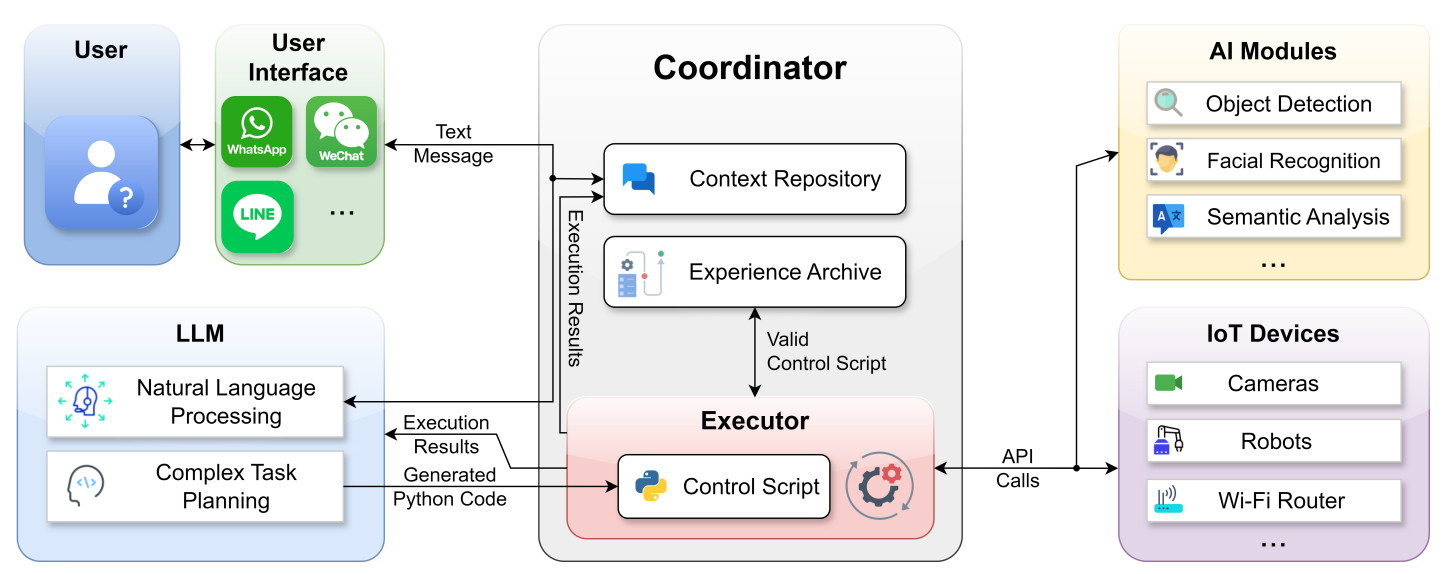
\includegraphics[width=0.6\textwidth]{./img/system_diagram.png} % 这里替换为图像文件名
  \caption{System diagram}
  \label{fig:llmFramwork}
\end{figure*}

% - - - - - - - - - - - - - - - - - - - - - - - - - - - - - - - - - - -
\section{Questions or Hypotheses}
\label{sec:questions}
Below are posed to optimize network detection based on their designed IIoT task-oriented framework,
which may help identify potential challenges, define research directions,
and evaluate the actual performance of the model.

\subsection{Fine-tuning Model}
% Model Adaptability
Firstly, Can a large model, once fine-tuned, adapt to different IIoT devices?
In which device environments does it perform best?
I think that fine-tuning a large model significantly improves
the accuracy and recall rates of IIoT network anomaly detection,
making it better suited for complex anomaly patterns than traditional detection methods.

% Model Scalability
On the other hand, the model flexibly adapt to emerging IIoT anomaly patterns,
or does it require periodic fine-tuning or retraining?
We can hypothesize that multi-task fine-tuning (e.g., anomaly detection and classification in parallel)
can further improve the model’s ability to identify specific types of anomalies.

\subsection{Data Processing}
% Data Requirements
Some questions that arise when we collect IIoT data is:
Does fine-tuning an IIoT anomaly detection model require a large amount of data?
How do data scale and quality impact detection effectiveness?
A moderate amount of IIoT anomaly data can greatly improve the model's generalization ability,
enabling it to maintain high detection accuracy across various IIoT environments.

% Knowledge Base \& RAG Vector Database
In Figure~\ref{fig:fsmProcedure}, if the RAG vector library and knowledge base are added,
can the command problems of the system be better located?
establishing this node requires additional resources.
Because in the industrial Internet of Things,
the environment that isolates the external network needs to be considered,
it is necessary to establish its own LLM independently.
Compared with the resources consumed by running LLM,
a vector library can be added to speed up the troubleshooting process.

\begin{figure} % [h] 表示将图像放置在此处
  % \centering
  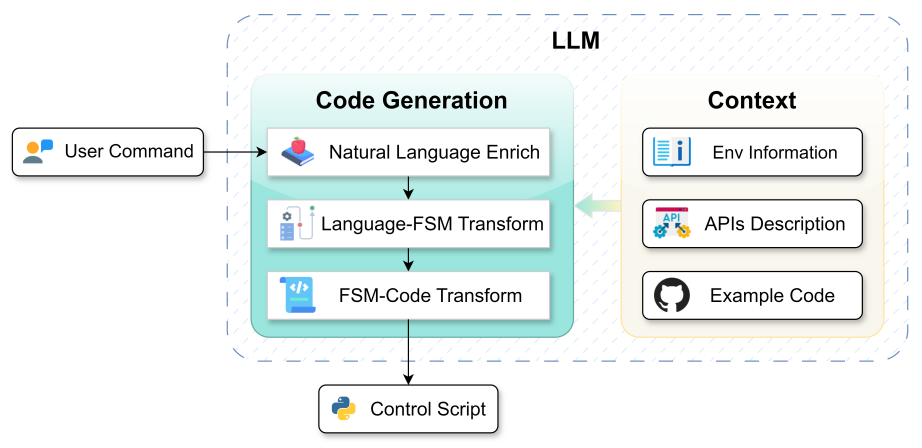
\includegraphics[width=0.5\textwidth]{./img/language_code_trans_procedure.png} % 这里替换为图像文件名
  \caption{Language-Code transformation procedure}
  \label{fig:fsmProcedure}
\end{figure}

% Data Privacy
However, Data privacy is a serious and unavoidable issue.
How can IIoT data privacy be effectively protected
during data collection and model deployment?
The fine-tuned model is suitable for real-time anomaly detection,
with a response time of 1-2 seconds for most IIoT network anomalies.

\subsection{Performance and Cost}
% Real-time Detection
About Performance, can the fine-tuned model meet real-time detection requirements
in practical applications? If there is latency,
how can it be optimized?
I assume that the false positive rate of a fine-tuned large model will be
substantially lower than traditional statistical or rule-based methods,
thereby reducing interference in anomaly detection.

% False Positive and False Negative Rates
Then, we need to seriously think about the cost issue.
What are the computational, storage, and energy costs when deploying
the fine-tuned model in IIoT environments?
Can it effectively operate on resource-limited devices?
Distributed fine-tuning can effectively reduce the computational
burden on IIoT devices without significantly impacting
detection performance.

% Resource Consumption
What are the computational, storage, and energy costs when
deploying the fine-tuned model in IIoT environments?
Can it effectively operate on resource-limited devices?
The model’s accuracy in detecting new types of anomalies will degrade over time,
but incremental fine-tuning can restore performance.

% - - - - - - - - - - - - - - - - - - - - - - - - - - - - - - - - - - -
\section{Methodology}
\label{sec:methodology}
The research will follow a systematic approach to develop and evaluate
the proposed anomaly detection framework.
The methodology includes the following steps.

\subsection{Technical Selection}

Models suitable for handling time series, such as T5, GPT,
or transformer-based time series models,
can be selected and fine-tuned for IoT data.
As shown in Table~\ref{tab:comparison}, Fine-tune the model using labeled normal/abnormal
IoT network data to enable the model to recognize common anomaly patterns.

\begin{table*}
  \centering
  \caption{Comparison of Different Methods}
  \label{tab:comparison}
  \begin{tabularx}{\textwidth}{>{\raggedright\arraybackslash}p{2.5cm} X X X}
      \toprule
      \textbf{Feature} & \textbf{LoRA} & \textbf{RLHF} & \textbf{MoE} \\
      \midrule
      \textbf{Method Type} & Parameter-efficient fine-tuning. & Training optimization. & Model architecture. \\
      \textbf{Core Goal} & Efficiently fine-tune the model. & Enhance the quality of generated content through human feedback. & Improve model performance through selective activation. \\
      \textbf{Suitable Scenarios} & High task adaptability, minimal parameter adjustments needed. & User interaction, dialogue systems. & Multi-task learning, handling complex inputs. \\
      \textbf{Advantages} & Resource-saving, lightweight fine-tuning. & Aligns with human preferences, high-quality output. & Large parameter count but controlled computational load. \\
      \textbf{Implementation} & Low-rank matrix insertion. & Reward model + reinforcement learning. & Mixture of experts network + sparse activation. \\
      \textbf{Cost} & Relatively low. & Relatively high. & High. (but less computation during inference) \\
      \textbf{Complexity} & Low. & High.(involves human feedback and reinforcement learning) & High.(requires expert selection and sparse activation) \\
      \bottomrule
  \end{tabularx}
\end{table*}

% RLHF
Further fine-tune the model using expert feedback after initial fine-tuning to optimize sensitivity to anomaly detection.
The reward model for RLHF has proven effective in fine-tuning Large Language Models
(LLMs)\citep{zhang2024prototypical}.
% LoRA
SLoRA(2024) observe that this paradigm presents significant opportunities
for batched inference during serving\citep{sheng2024slora}.
So, we use LoRA for lightweight fine-tuning to save resources.

% MoE
MoE combines different experts (i.e., sub-models or networks)
with the aim of activating only a subset of these "experts" based
on the specific needs of the input task.
LLM-HAS innovative framework leverages a Mixture
of Experts (MoE) approach, augmented with LLMs, to analyze
users’ personalized preferences and potential health risks from
additional textual job descriptions\citep{gao2024guiding}.

Furthermore, the Hugging Face Transformers library and Datasets API can be utilized for
managing datasets and model fine-tuning tasks,
while DeepSpeed can be employed for distributed training and deployment.
It serves as a versatile framework that offers flexible fine-tuning tools.
However, techniques such as LoRA, RLHF, and MoE are more targeted approaches
designed for specific fine-tuning needs and scenarios.
Therefore, I don't choose the Transformers library as the tool for fine-tuning
large models in this context.

\subsection{Data Preparation}

Gather traffic, logs, and sensor data from IoT devices over a period.
Focus on collecting and labeling anomalies and normal events occurring
in actual network environments.

Then, extract features (e.g., traffic peaks, connection frequencies, packet sizes)
from the data and remove noise. Data augmentation techniques can be
used to expand anomaly samples.

Finally, organize data into time series input formats,
such as sliding window sequences, for the model to learn
inter-event relationships.

\subsection{Fine-Tuning Model}

We will select an appropriate LLM and fine-tune it on the collected IIoT data. As mentioned in the work of
\citet{sarabi2023llm}.First fine-tune the model using general network data to learn basic network patterns,
then use IoT-specific data for further fine-tuning to learn specific patterns.

Implement multi-task learning to enable the model to perform anomaly detection while also
classifying types of anomalies (e.g., identifying DDoS attacks, packet loss).

\subsection{Evaluation and Validation}

The fine-tuned LLM will be trained on the IIoT dataset, and its performance will be
validated using a separate validation set to ensure the model's effectiveness in detecting anomalies.
Compare with traditional detection models (e.g., rule-based or statistical analysis methods) to analyze
the advantages and shortcomings of the fine-tuned large model.

The performance of the fine-tuned LLM will be compared with traditional anomaly detection methods to
evaluate its improvement in accuracy and efficiency.
The model will be deployed in a real-world IIoT network setting to test its practical
applicability and robustness in various operational scenarios.

% - - - - - - - - - - - - - - - - - - - - - - - - - - - - - - - - - - -
\section{Expected Outcomes and Contributions}
\label{sec:outcomes}
We anticipate establishing a new IIoT framework that enhances resilience against
potential threats and anomalies in existing IIoT network security.
This framework aims to improve the effectiveness of industrial IIoT
security through validated evidence, contributing to the knowledge
base of this emerging field.

With fine-tuned LLMs demonstrating their versatility beyond
natural language tasks in industrial contexts, we expect the model
to achieve higher accuracy and recall rates after fine-tuning,
with an anticipated increase of 5-10\% in accuracy.
The model will adapt more swiftly to new or complex anomalies,
thereby expanding its capability to detect various types of
attacks or anomalies.

Finally, we will maintain the model’s adaptability to
emerging IIoT anomalies through regular fine-tuning or
the incorporation of new data.

% - - - - - - - - - - - - - - - - - - - - - - - - - - - - - - - - - - -
\section{Conclusion}
\label{sec:conclusion}
In this research plan, I analyze the current state of research on the integration
of IIoT and LLMs in the fields of monitoring and control.
Recent studies on IIoT device control have utilized OpenAI
to generate control code for these devices.

I propose a framework for fine-tuning large models to
enhance the detection of network anomalies in IoT devices
that integrate LLM control systems. Frameworks such as LoRA,
RLHF, and MoE, which are tailored for specific scenarios,
can effectively address troubleshooting in network anomaly
situations, thereby reducing time costs and improving efficiency.

Additionally, it is essential to consider data collection and
significant cost factors. Ultimately, the goal is to achieve a
5-10\% increase in efficiency, improving the control framework
for industrial IoT research.
% - - - - - - - - - - - - - - - - - - - - - - - - - - - - - - - - - - -
\bibliographystyle{tjaa}
\bibliography{Example}

% \newpage\newpage
% - - - - - - - - - - - - - - - - - - - - - - - - - - - - - - - - - - -
% \section{Fine tuning the manuscript}

% A new command is introduced to collect all astronomical objects into a
% database:
% \verb|\Aobj{Cyg X-1}|.
% The following code
% ``\verb|Andromeda galaxy (\Aobj{M31}) ...|''
% will produce
% ``Andromeda galaxy (\Aobj{M31}) ...''
% and the object (M31) will be added to the object database.

% Links to web pages can be given within the text using \verb|\url| command:
% The command \verb|\url{https://tad.org.tr}| will produce
% \url{https://tad.org.tr}.
% For longer URLs you can merge the URL into text using the web format.
% The command
% \verb|\href{https://dergipark.org.tr/tjaa}{TJAA}|\\
% will produce a link to \href{https://dergipark.org.tr/tjaa}{TJAA}.

% Some of the common commands, properties and habits:
% \begin{flushleft}
% \begin{tabular}{@{}p{.15\columnwidth}p{.75\columnwidth}}
% \verb|\,|   & a thin space, e.g.\ between numbers or between units
%               and numbers; a line division will not be made
%               following this space\\
% \verb|--|   & en dash; two strokes, without a space at either end;
% 	      put in between numbers to increase readability\\
% \verb*| -- |& en dash; two strokes, with  a space at either end\\
% \verb|-|    & hyphen; one stroke, no space at either end\\
% \verb|$-$|  & minus, in the text {\em only} \\
% {\em Input} & \verb|21\,$^{\circ}$C etc.,|\\
%             & \verb|Dr h.\,c.\,Rockefellar-Smith \dots|\\
%             & \verb|1950--1985 \dots|\\
%             & \verb|this -- printed on a computer|\\
% {\em Output}& 21\,$^{\circ}$C etc., Dr h.\,c.\,Rockefellar-Smith \dots\\
%             & 1950--1985 \dots\\
%             & this -- printed on a computer
% \end{tabular}
% \end{flushleft}

% % - - - - - - - - - - - - - - - - - - - - - - - - - - - - - - - - - - -
% \section{Special text typefaces}

% Normal type (roman text) need not be coded. Three different command
% emphasizes the text:
% \begin{flushleft}
% \begin{tabular}{@{}p{.32\columnwidth}p{.6\columnwidth}}
% \verb|{\itshape Text}|   & {\itshape Italicized Text}\\
% \verb|{\em Text}|   & {\em Emphasized Text --
%    if you would like to emphasize a {\em definition} within an
%    italicized text (e.g.\ of a {\em theorem}) you should code the
%    expression to be emphasized by} \verb|\em|.\\
% \verb|{\bfseries Text}|& {\bfseries Important Text}\\
% \verb|\vec{Symbol}| & Vectors may only appear in math mode. The default
%    \LaTeX{} vector symbol has been adapted\footnotemark\
%    to LLNCS conventions.\\[2pt]
%  & \verb|$\vec{A \times B\cdot C}|\\
%  & ... yields $\vec{A\times B\cdot C}$
% \end{tabular}
% \end{flushleft}
% %\footnotetext{If you absolutely must revive the original \LaTeX{}
% %design of the vector symbol (as an arrow accent), please specify the
% %option \texttt{[orivec]} in the \texttt{documentclass} line.}

% % - - - - - - - - - - - - - - - - - - - - - - - - - - - - - - - - - - -
% \section{Astronomical Macros}

% List of short cuts for astronomy. Note that all of the macros listed below are
% math mode safe i.e. \verb|$12\degr$| and \verb|12\degr| will produce the same
% text.
% \begin{flushleft}
% \begin{large}
% \begin{tabular}{@{}p{.50\columnwidth}@{~}p{.40\columnwidth}@{}}
% \verb|12 \fd     34\fh     56| & $12\fd34\fh56$ \\
% \verb|12 \fm     34\fs     56| & $12\fm34\fs56$ \\
% \verb|12 \fdg    34\fas    56| & $12\fdg34\fas56$ \\
% \verb|12 \fp     3456        | & $12\fp3456$ \\
% \verb|12 \farcm  34\farcs  56| & $12\farcm34\farcs56$ \\
% \verb|12 \arcmin 34\arcsec 56| & 12\arcmin34\arcsec56 \\
% \end{tabular}
% \end{large}
% \end{flushleft}
% \newpage
% \begin{flushleft}
% \begin{large}
% \begin{tabular}{@{}p{.50\columnwidth}@{~}p{.50\columnwidth}@{}}
% \verb|1\degr                | & 1\degr \\
% \verb|1\Fd  2\Fh  3\Fm  4\Fs| & $1\Fd 2\Fh 3\Fm 4\Fs$ \\
% \verb|1\Fdg 2\Fam 3\Fas     | & $1\Fdg 2\Fam 3\Fas$ \\
% &\\[-2pt]
% \verb|1 {M,R,L,T}\solarxxx  | & $1\solarmass 1\solarrad 1\solarlum 1\solartemp$ \\
% \verb|1 {unit}\perxxx       | & g\perone m\persq s\percube \\
% \verb|\renkBV \renkEBV      | & $\renkBV=\renkEBV$ \\
% \verb|\renkUB \renkEUB      | & $\renkUB=\renkEUB$ \\
% \verb|12 \micron \ion{H}{II}| & $12\micron$ \ion{H}{II} \\
% \end{tabular}
% \end{large}
% \end{flushleft}

% % - - - - - - - - - - - - - - - - - - - - - - - - - - - - - - - - - - -
% \section{Astronomical Journals}

% List of journal abbreviations used in TJAA references. Note that to fit into
% the page only a partial list shown here.
% \begin{verbatim}
% \aap \aapr \aaps \aat \actaa \afz \aj \ao \apj
% \apjl \apjs \aplett \apss \araa \arep \aspc \azh
% \baas \caa \cjaa \iaucirc \icarus \japa \jrasc
% \mnras \na \nar \nat \pasa \pasj \pasp \planss
% \procspie \qjras \rmxaa \sci \skytel \solphys
% \sovast \ssr \tjaa \an \psj          \vark
% \end{verbatim}
% \begin{footnotesize}
% \aap		~$\bullet$
% \aapr		~$\bullet$
% \aaps		~$\bullet$
% \aat		~$\bullet$
% \actaa		~$\bullet$
% \afz		~$\bullet$
% \aj		~$\bullet$
% \ao 		~$\bullet$
% \apj		~$\bullet$
% \apjl		~$\bullet$
% \apjs		~$\bullet$
% \aplett		~$\bullet$
% \apss		~$\bullet$
% \araa		~$\bullet$
% \arep		~$\bullet$
% \aspc		~$\bullet$
% \azh		~$\bullet$
% \baas		~$\bullet$
% \caa		~$\bullet$
% \cjaa		~$\bullet$
% \iaucirc	~$\bullet$
% \icarus		~$\bullet$
% \japa		~$\bullet$
% \jrasc		~$\bullet$
% \mnras		~$\bullet$
% \na		~$\bullet$
% \nar		~$\bullet$
% \nat		~$\bullet$
% \pasa		~$\bullet$
% \pasj		~$\bullet$
% \pasp		~$\bullet$
% \planss		~$\bullet$
% \procspie	~$\bullet$
% \qjras		~$\bullet$
% \rmxaa		~$\bullet$
% \sci		~$\bullet$
% \skytel		~$\bullet$
% \solphys	~$\bullet$
% \sovast		~$\bullet$
% \ssr		~$\bullet$
% \an		~$\bullet$
% \psj		~$\bullet$
% \tjaa\\\vark
% \end{footnotesize}

% % - - - - - - - - - - - - - - - - - - - - - - - - - - - - - - - - - - -
% \section{Footnotes}

% \paragraph*{\itshape Sample Input}~\\
% Text with a footnote\verb|\footnote{The |{footnotes are numbered automatically.}\verb|}| and text continues \dots

% \paragraph*{\itshape Sample Output}~\\
% Text with a footnote\footnote{The footnotes are numbered automatically.}
% and text continues \dots

% % - - - - - - - - - - - - - - - - - - - - - - - - - - - - - - - - - - -
% \section{Lists}

% \paragraph*{\itshape Sample Input}
% \begin{verbatim}
% \begin{enumerate}
%   \item First item
%   \begin{enumerate}
%     \item First nested item
%   \end{enumerate}
%   \item Second item
% \end{enumerate}
% \end{verbatim}
% \paragraph*{\itshape Sample Output}
% \begin{enumerate}
%   \item First item
%   \begin{enumerate}
%     \item First nested item
%   \end{enumerate}
%   \item Second item
% \end{enumerate}

% % - - - - - - - - - - - - - - - - - - - - - - - - - - - - - - - - - - -
% \newpage
% \section{Floating environments: Figures \& Tables}
% \begin{lrbox}{\verbbox}
% \verb|\protect\citep{author2021}|
% \end{lrbox}

% They should be inserted after (not in) the  paragraph in which the figure is
% first mentioned.
% They will be numbered automatically.
% Note that figures (and tables) become floating environments if they are not
% attached to main text.
% Therefore if you want to place the figure (or table) correctly
% \textbf{do not add empty lines} before \verb|\begin{figure}| or
% \verb|\begin{table}|.

% If you have many floating blocks (figures or tables) you have two choices:
% \begin{enumerate}
% \item
% Push all floats to the end \textbf{with no space between the blocks} in the
% same order as they are referenced;
% \item
% Start arranging the location of floats from the very first float putting and
% fixing its location couple of paragraphs before it is referenced first. This
% way the floats will be -/+ 1 one page away from its expecting location.
% \end{enumerate}
% The image file formats are limited to only PNG or PDF types.

% \subsection{Figures}

% To leave the desired amount of space for the height of your figures, please
% use the coding described below.
% Please note that ``\verb|x|'' in the following coding stands for the actual
% height of the figure:
% \begin{verbatim}
% \begin{figure}
% \vspace{x cm}
% %              (Use [ ] for short caption)
% \caption[ ]{...text of caption...}
% \end{figure}
% \end{verbatim}
% \paragraph*{\itshape Sample Input}
% \begin{verbatim}
% \begin{figure}
% \vspace{2.5cm}
% \caption{This is the caption of the figure
% displaying nothing leaving a vertical space
% of 2.5 cm.
% If you need to use cited references in
% caption use \protect command:
% \protect\citep{author2021}.}
% \end{figure}
% \end{verbatim}
% \paragraph*{\itshape Sample Output.}{\itshape Figure is placed at the top of the column} 
% \begin{figure}
% \vspace{2.5cm}
% \caption{%
% This is the caption of the figure displaying nothing leaving a vertical space
% of 2.5 cm. If you need to use cited references in caption use the following
% command: \usebox{\verbbox}.}
% \end{figure}

% % - - - - - - - - - - - - - - - - - - - - - - - - - - - - - - - - - - -
% \newpage
% \subsection{Tables}

% Table captions should be treated in the same way as figure legends, except
% that the table captions appear {\itshape above} the tables. 
% \paragraph*{\itshape Sample Input}
% \begin{verbatim}
% \begin{table}
% \caption{Critical $N$ values}
% \begin{tabular}{rllllL{7mm}@{}C{7mm}@{}R{7mm}}
% \hline     % No need to use \noalign{\smallskip}
% ${\mathrm M}_\odot$
%   & $\beta_{0}$ & $T_{\mathrm c6}$ & $\gamma$
%   & $N_{\mathrm{crit}}^{\mathrm L}$
%   & L & C & R \\
% \hline
% % You dont need to use      \noalign{\smallskip}
% % around the \hline command.
% % It is provided internally.
%  30 & 0.82 & 38.4 & 35.7 & 154 &1   &1    &1  \\
%  60 & 0.67 & 42.1 & 34.7 & 138 &12  &12   &12 \\
% 120 & 0.52 & 45.1 & 34.0 & 124 &123 &123  &123\\
% \hline
% \end{tabular}
% \end{table}
% \end{verbatim}
% \paragraph*{\itshape Sample Output:}
% Table is placed at the top of this column. To place flowing text
% correctly, start a new paragraph by pressing enter twice after the table.
% \begin{table}
% \caption{Critical $N$ values}
% \centering
% % Please dont use commands giving extra vertical or horizontal spacing.
% % They are all deleted or converted to publisher standards.
% \begin{tabular}{rllllL{7mm}@{}C{7mm}@{}R{7mm}}
% % When \tabcolsep is used your table will take more space than expected.
% %\setlength\tabcolsep{3pt}
% \hline
% ${\mathrm M}_\odot$
%   & $\beta_{0}$ & $T_{\mathrm c6}$ & $\gamma$
%   & $N_{\mathrm{crit}}^{\mathrm L}$
%   & L & C & R \\
% \hline
%  30 &0.82 &38.4 &35.7 &154 &1   &1   &1  \\
%  60 &0.67 &42.1 &34.7 &138 &12  &12  &12 \\
% 120 &0.52 &45.1 &34.0 &124 &123 &123 &123\\
% \hline
% \end{tabular}
% \end{table}

% Two important notes:
% (1) 4 new columntypes introduced (P, L, C, R) -- last three
% shown here.
% For example \verb|C{1cm}| centers the content of the column to 1 cm width.
% (2) If you use \verb|dcolumn| option for \verb|tjaa| style, 3 new column types
% (namely, \verb|d . ,|) can be used to align the numbers in the column content.

% For further information you will find a complete description of the tabular
% environment on p.~62~ff. and p.~204 of the {\em \LaTeX{} User's Guide \&
% Reference Manual\/} by Leslie Lamport.

% % - - - - - - - - - - - - - - - - - - - - - - - - - - - - - - - - - - -
% \section{Symbols and Characters}

% \subsection*{Special Symbols}

% You may need to use special signs.  The available ones are listed in the {\em
% \LaTeX{} User's Guide \& Reference Manual\/} by Leslie Lamport, pp.~41\,ff. We
% have created further symbols for math mode (enclosed in \$):
% \begin{center}
% \begin{tabular}{l@{\hspace{1em}yields\hspace{1em}}
% c@{\hspace{3em}}l@{\hspace{1em}yields\hspace{1em}}c}
% \verb|\grole| & $\grole$ & \verb|\getsto| & $\getsto$\\
% \verb|\lid|   & $\lid$   & \verb|\gid|    & $\gid$
% \end{tabular}
% \end{center}
% \newpage

% % - - - - - - - - - - - - - - - - - - - - - - - - - - - - - - - - - - -
% \section{Acknowledging other parties}

% Scientific works usually have to acknowledge many different institutions,
% works, individuals, software etc.
% In a proper acknowledgment, these should be listed according to the
% importance and contribution, starting from highest to lowest, and group them:
% projects, software, institutions, people.

% Note also that acknowledgment section is not numbered and should be the last
% section before references:
% \paragraph*{\itshape Sample Input}
% \begin{verbatim}
% \section*{Acknowledgment}
% \end{verbatim}

% \section{Required Disclosures}
% Authors are now required to disclose two extra information: (1) Conflict of
% Interest, and (2) Contribution Percentage among the authors. Authors should
% typeset the following section after the acknowledgement. Note that, the
% following Turkish equivalents should be used for Turkish text, in order of
% apparance: Açıklamalar, Çatışma Beyanı, Katkı Oranı.
% \begin{verbatim}
% \section*{Disclosures}
% \paragraph{Conflict of Interest:} All authors
% declare that they have no conflicts of interest.
% \paragraph{Contribution:} All authors contributed
% equally in writing the manuscript.
% \end{verbatim}

% If authors have conflict of interests then they could use the following
% conflict of interest templates as examples:
% \begin{verbatim}
% - X has received a research grant from FIRM. 
% - X is an employee of FIRM.
% - X received part time salary for this work.
% - X is on board of JOURNAL.
% - X has a patent pending for PATENT.
% - X declares no conflicts of interest.
% \end{verbatim}

% % - - - - - - - - - - - - - - - - - - - - - - - - - - - - - - - - - - -
% \section{References}
% \label{refer}

% There are two ways to enter citations in \LaTeX{}:
% (1) Citing with plain text inline in the manuscript using
% \textit{pre-formatted list of references};
% (2) Referring to a permanent database of references and calling with BibTeX
% tools.
% We recommend the later one to our colleagues, especially if you are a beginner
% in writing scientific papers.
% In this manuscript both of them will be explained.

% There are three different citation presentation exists.
% However, in this manuscript, only ``Author-Year'' style which is widely
% used in astronomy, will be explained and therefore implemented in TJAA.
% The other two are: number only and letter--number.

% Entering citations and typesetting references are explained in
% ``{\em \LaTeX{} User's Guide \& Reference Manual\/}, Leslie Lamport, s.~71.''
% In this manuscript only a simplified will be used.

% \newpage
% \subsection{Author-Year System}

% Referenced cited within the text in parenthesis which contains author and
% year.
% Some of the examples of this usage are as follows:
% (Smith 1970, 1980), (Ekeland et al. 1985, Theorem 2), (Jones and Jaffe
% 1986; Farrow 1988, Chap.\,2).
% If the author is part of the text only the year could be put into the
% parenthesis:
% eg.\ Ekeland et.al.\ (1985, Section.\,2.1)
% Reference list should include all the cited word and it has to be order with
% the surname.
% If there are more than one work for the same author then they should be listed
% with the following rules:
% \begin{enumerate}
% \setlength{\hfuzz}{5pt}
% \item
% Single Author: List is sorted by date.
% \item
% Author and the same other authors: List is sorted by date.
% \item
% Author and different other authors: List has to be sorted alphabetically by
% the other authors.
% \end{enumerate}
% If there are more than one cited work for the same author(s) then each work
% has to be suffixed with sequential letter, ``a'', ``b'' etc.
% eg.\ (Smith 1982a), (Smith 1982b), (Ekeland et al. 1982c).

% \subsection{Author-Year commands}

% For the following \verb|\bibitem[]{}| command created by BibTeX the following
% list of citation usage is available through out the manuscript:\\
% \verb|\bibitem[Auth1 et al. (2021)Auth1, Auth2,|\\
% \verb|    and Auth3]{key21}...|
% \small
% \begin{flushleft}
% \begin{tabular}{@{}p{.45\columnwidth}@{~}p{.50\columnwidth}@{}}
% \verb|\citet{key21}|       & Auth1 et al. (2021) \\
% \verb|\citep{key21}|       & (Auth1 et al., 2021) \\
% \verb|\citet*{key21}|      & Auth1, Auth2, and Auth3 (2021) \\
% \verb|\citep*{key21}|      & (Auth1, Auth2, and Auth3, 2021) \\
% & \\
% \verb|\citet[txt1]{key21}| & Auth1 et al. (2021, txt1) \\
% \verb|\citep[txt1]{key21}| & (Auth1 et al., 2021, txt1) \\
% \verb|\citep[txt1][]{key21}| & (txt1 Auth1 et al., 2021) \\
% \verb|\citep[txt1][txt2]{key21}| & (txt1 Auth1 et al., 2021, txt2) \\
% & \\
% \verb|\citealt{key21}|     & Auth1 et al. 2021 \\
% \verb|\citealp{key21}|     & Auth1 et al., 2021 \\
% \verb|\citealt*{key21}|    & Auth1, Auth2, and Auth3 2021 \\
% \verb|\citealp*{key21}|    & Auth1, Auth2, and Auth3, 2021 \\
% & \\
% \verb|\citetext{priv.\ comm.}| & (priv. comm.) \\
% \end{tabular}
% \end{flushleft}
% \normalsize

% \textbf{This system has been integrated into TJAA style and you don't need to
% change anything in your manuscript; just continue using your habit of citing.}

% \begin{center}
% \Large\textbf{IMPORTANT NOTE:}\\
% Below  you will find two different methods.\\
% Choose one type of citing and referencing and\\
% delete the other section completely.
% \end{center}

% \newpage
% \subsection{Author-Year: Inline with text}

% You have to assign an alias (embraced with curly brackets) to each reference
% you put in `References' section with \verb|\bibitem| command.
% You then use \verb|\cite{alias}| command to refer to the reference
% inline within the text.

% Note that in this `inline' method, author has full control of the format of
% \verb|\bibitem|. However, since entries are written and maintained by hand,
% copy-pasting from other source files might create inconsistencies which would
% not easy to resolve for large number of entries.

% \paragraph*{\itshape Example-1 -- Citing a reference: Input}
% \begin{verbatim}
% The results in this section are a
% refined version of \citet{clar:eke1}; the
% minimality result of Proposition~14 was the
% first of its kind.
% \end{verbatim}

% \paragraph*{\itshape Example-1 -- Citing a reference: Output}
% ``\dots\ refined version of \citet{clar:eke1}; the minimality\dots''.

% \paragraph*{\itshape Example-1 -- Building References: Input}
% \begin{verbatim}
% %      (don't forget {} string at the end)
% \begin{thebibliography}{}
% .
% .
% \bibitem[Clarke ve Ekeland, 1982]{clar:eke1}
% Clarke, F., Ekeland, I.:
% Nonlinear oscillations and boundary-value
% problems for Hamiltonian systems.
% Arch. Rat. Mech. Anal. {\bfseries 78} (1982)
% 315--333
% .
% .
% \end{thebibliography}
% \end{verbatim}

% \paragraph*{\itshape Example-1 -- Building References: Output}
% %%%%TJAA-OZEL:BIB%
% \begin{thebibliography}{}
% \bibitem[Clarke ve Ekeland, 1982]{clar:eke1} Clarke, F., Ekeland, I.: Nonlinear
% oscillations and boundary-value problems for Hamiltonian systems.
% Arch. Rat. Mech. Anal. {\bf 78} (1982) 315--333
% \end{thebibliography}

% \newpage
% \subsection{Author-Year: with {\sc Bib}\TeX{}}

% The only difference of this method from the \textit{inline} method is that
% \verb|\bibitem| lines are generated automatically using an external command
% (\verb|bibtext|).
% Therefore, format of \verb|\bibitem| lines will also be standard too.
% The standard for TJAA is adapted from Springer's {\sc Bib}\TeX{} style and it
% is available through \verb|tjaa.bst| file and the command
% \verb|\bibliographystyle{tjaa}| will handle the rest of the configuration.

% Citation in this example will be exactly the same as in the previous one.

% \paragraph*{\itshape Example-2 -- Citing a reference: Input}
% \begin{verbatim}
% The results in this section are a
% refined version of \citet{clar:eke2}; the
% minimality result of Proposition~14 was the
% first of its kind.
% \end{verbatim}

% \paragraph*{\itshape Example-2 -- Citing a reference: Output}
% ``\dots\ refined version of \citet{clar:eke2}; the minimality\dots''.

% \paragraph*{\itshape Example-2 -- Building References: Input}
% \begin{verbatim}
% \bibliographystyle{tjaa}
% \bibliography{Example}
% \end{verbatim}
% \paragraph*{\itshape Example-2 -- Building References: Input} \verb|Example.bib| file.
% \begin{verbatim}
% @ARTICLE{clar:eke2,
%  author  = {{Clarke}, F. and {Ekeland}, I.},
%  title   = "{Nonlinear ... systems.}",
%  journal = {Arch. Rat. Mech. Anal.},
%  year    = 1982,
%  volume  = 78,
%  pages   = {315-333},
%  tjaanote= {Prepared for TJAA example.
%             Note: Even though each keyword=value
%             ends with comma in previous lines,
%             this line doesnt.}
% }
% \end{verbatim}
% \paragraph*{\itshape Example-2 -- Building References: Output}
% %%%%TJAA-OZEL:BIB%
% % \bibliographystyle{tjaa}
% % \bibliography{Example}

% \subsection{Future of Bibliography Management}

% Users might find it to difficult to maintain a bibliographic reference list in
% a special formatted file with \verb|.bib| extension.
% However, nowadays all bibliographical databases provide \verb|.bib| outputs.
% Then, you just have to refer to these files using the following command:
% \verb|\bibliography{tjaa2021}|.

% Even though maintaining ``a reference database'' means to combine a few
% different concepts together, once it is done for the first time, later usage
% would be handled by combining different \verb|.bib| files in a
% single command. For example, use the following command to combine your
% previous TJAA submissions:
% \verb|\bibliography{tjaa-M1,tjaa-2018,tjaa-2021}|.

% In today's capabilities, please consider exporting your bibliographical
% databases stored in \verb|.bib| files into a modern style software; one of
% which is
% \href{https://zotero.org/}{Zotero} and it is also integrated in
% \href{https://overleaf.com/}{Overleaf}, a web based tool to collaboratively
% write in \LaTeX{}, store, share and produce articles.
% TJAA style is available in \href{https://overleaf.com/}{Overleaf}.

%%%%TJAA-OZEL:SON%
\label{lastpage}
\end{document}
